%\VignetteIndexEntry{Pairwise Sequence Similarity Simple}
%\VignetteDepends{}
%\VignetteKeywords{Sequence analysis}
%\VignettePackage{pairseqsim}

\documentclass{article}

\title{Pairwise Sequence Similarity Simple}
\author{Witold Eryk Wolski}

\usepackage{/loc/biocbuild/1.9d/R/share/texmf/Sweave}
\begin{document}

\maketitle
\setkeys{Gin}{width=0.7\textwidth}

\section{Introduction}

The first fact of biological sequence analysis: In bio-molecular sequences (DNA, RNA, or amino acid sequences), high sequence similarity usually implies significant functional or structural similarity. The \texttt{pairseqsim} package can be used to compute pairwise sequence alignments of two amino acid sequences. Based on the optimal alignment of two sequences it computes also basic scores like sequence similarity, identity, and the alignment score. The optimal alignment can be visualized. A distance matrix storing all pairwise distances of all sequences in list can be computed. This matrix can be used to cluster the sequences using various clustering algorithms provided by {\bf R}. 
To compute a biological meaningful alignment, a measure of amino acid similarity is needed. This information is provided by the families of BLOSUM or the PAM amino acid residue distance matrices. We imported many of this matrices from the EMBOSS software package (\texttt{http://www.hgmp.mrc.ac.uk/Software/EMBOSS/}. Gaps in an alignment are undesirable and thus penalized. The package implements an affine gap penalty:
\begin{equation}
\gamma(g)=d+(g-1)e
\end{equation}
where $d$ is the gap opening penalty and $e$ is the gap extension penalty.

The package implements three types of alignment:
\begin{itemize}
\item Global Alignment.
\item Local Alignment.
\item Overlap Alignment.
\end{itemize}

\emph{Global alignment} is applicable when we have two similar sequences that we want to align from end-to-end, e.g. two homologous genes from related species. To compute the global alignment the Needelman and Wunsch algorithm are used. For computing the \emph{local alignment} the Smith Waterman algorithm are used.  This type of alignment can be used if we would like to find the best match between subsequences of both. For example, we may want to find the position of a fragment of DNA in a genomic sequence. If we are given different fragments of genomic DNA that we would like to piece together, then we need an alignment method that does not penalize overhanging ends. Such an alignment can be computed by the \emph{overlap alignment}.

\section{Defining Sequences, Sequence Lists and Loading Data.}
First you have to load the package with

\begin{Schunk}
\begin{Sinput}
> library(pairseqsim)
\end{Sinput}
\end{Schunk}

If we want to analyze more than one pair of sequences we need to define a list (\texttt{AASequencelist}) which stores our sequence objects. 
\begin{Schunk}
\begin{Sinput}
> mySequlist <- new("AASequenceList", info = "my sequence list")
\end{Sinput}
\end{Schunk}
 
To the \texttt{AASequenceList} only an \texttt{AASequence} can be assigned. To define a new sequence we either use the \texttt{new} function or the function \texttt{AASequence}. The default constructor checks if the string is an amino acid sequence. This is done by comparing the letters in the sequence string to the amino acid alphabet which is defined by the class \texttt{AAAlphabet}. In the \texttt{AAAlphabet} class the characters which denote the amino acids are hard coded.

\begin{Schunk}
\begin{Sinput}
> new("AAAlphabet")
\end{Sinput}
\begin{Soutput}
info :  AminoAcid 
Alphabet :
 A R N D C Q E G H I L K M F P S T W Y V B Z X * 
\end{Soutput}
\end{Schunk}

\begin{Schunk}
\begin{Sinput}
> pseq <- "MRTNPTTSNPEVSIREKKNLGRIAQIIGPVLDVAFPPGKMPNIYNALVVK"
> access <- "MyatpB"
> myseq1 <- new("AASequence", pseq, info = access)
> myseq1 <- AASequence(access, pseq)
\end{Sinput}
\end{Schunk}

There are many protein sequence database formats. In this package only a reader for the \texttt{FASTA} file format is implemented (\texttt{readFasta}). The \texttt{FASTA} file format looks in the following way.

\begin{verbatim}
>At1g01010 NAC domain protein, putative
MEDQVGFGFRPNDEELVGHYLRNKIEGNTSRDVEVAISEVNICSYDPWNLRFQSKYKSRD
AMWYFFSRRENNKGNRQSRTTVSGKWKLTGESVEVKDQWGFCSEGFRGKIGHKRVLVFLD
GRYPDKTKSDWVIHEFHYDLLPEHQRTYVICRLEYKGDDADILSAYAIDPTPAFVPNMTS
S*
\end{verbatim}

Sequences in \texttt{FASTA} file format are preceded by a line starting with the symbol ``>'' as the first character. The rest of the line is the name and description of the sequence. The following lines contain the sequence data. To extract the ``info'' (id) string from the first line we define a function \texttt{infogrep} that extracts the appropriate substring from the line with the ``>''. We assign this function to the argument \texttt{grepinfo}. 

\begin{Schunk}
\begin{Sinput}
> infogrep <- function(x) {
+     return(sub("^>([a-zA-Z0-9]+) .+", "\\1", x, perl = TRUE))
+ }
\end{Sinput}
\end{Schunk}

Additionally a function can be defined which pre-processes the amino acid sequence. In many sequence databases the end of the sequence is denoted by ``*''. The function \texttt{seqgrep} which we assign to the parameter \texttt{grepseq} will remove it from the end of the sequence string.

\begin{Schunk}
\begin{Sinput}
> seqgrep <- function(x) {
+     return(gsub("\\*", "", x))
+ }
\end{Sinput}
\end{Schunk}

The first argument to the function \texttt{readFasta} are a object of class \texttt{AASequenceList}, the second are the path to the file.
\begin{Schunk}
\begin{Sinput}
> fdat <- system.file("test", package = "pairseqsim")
> mySequlist <- readFasta(mySequlist, paste(fdat, "ex.fasta", sep = "/"), 
+     grepinfo = infogrep, grepseq = seqgrep)
> length(mySequlist)
\end{Sinput}
\begin{Soutput}
[1] 66
\end{Soutput}
\end{Schunk}

\section{Analysing the Protein sequences}

To take a look at the amino acid composition of a protein sequence we use the function frequency.
%<<>>=
%barplot(frequency(mySequlist[[1]]))
%@
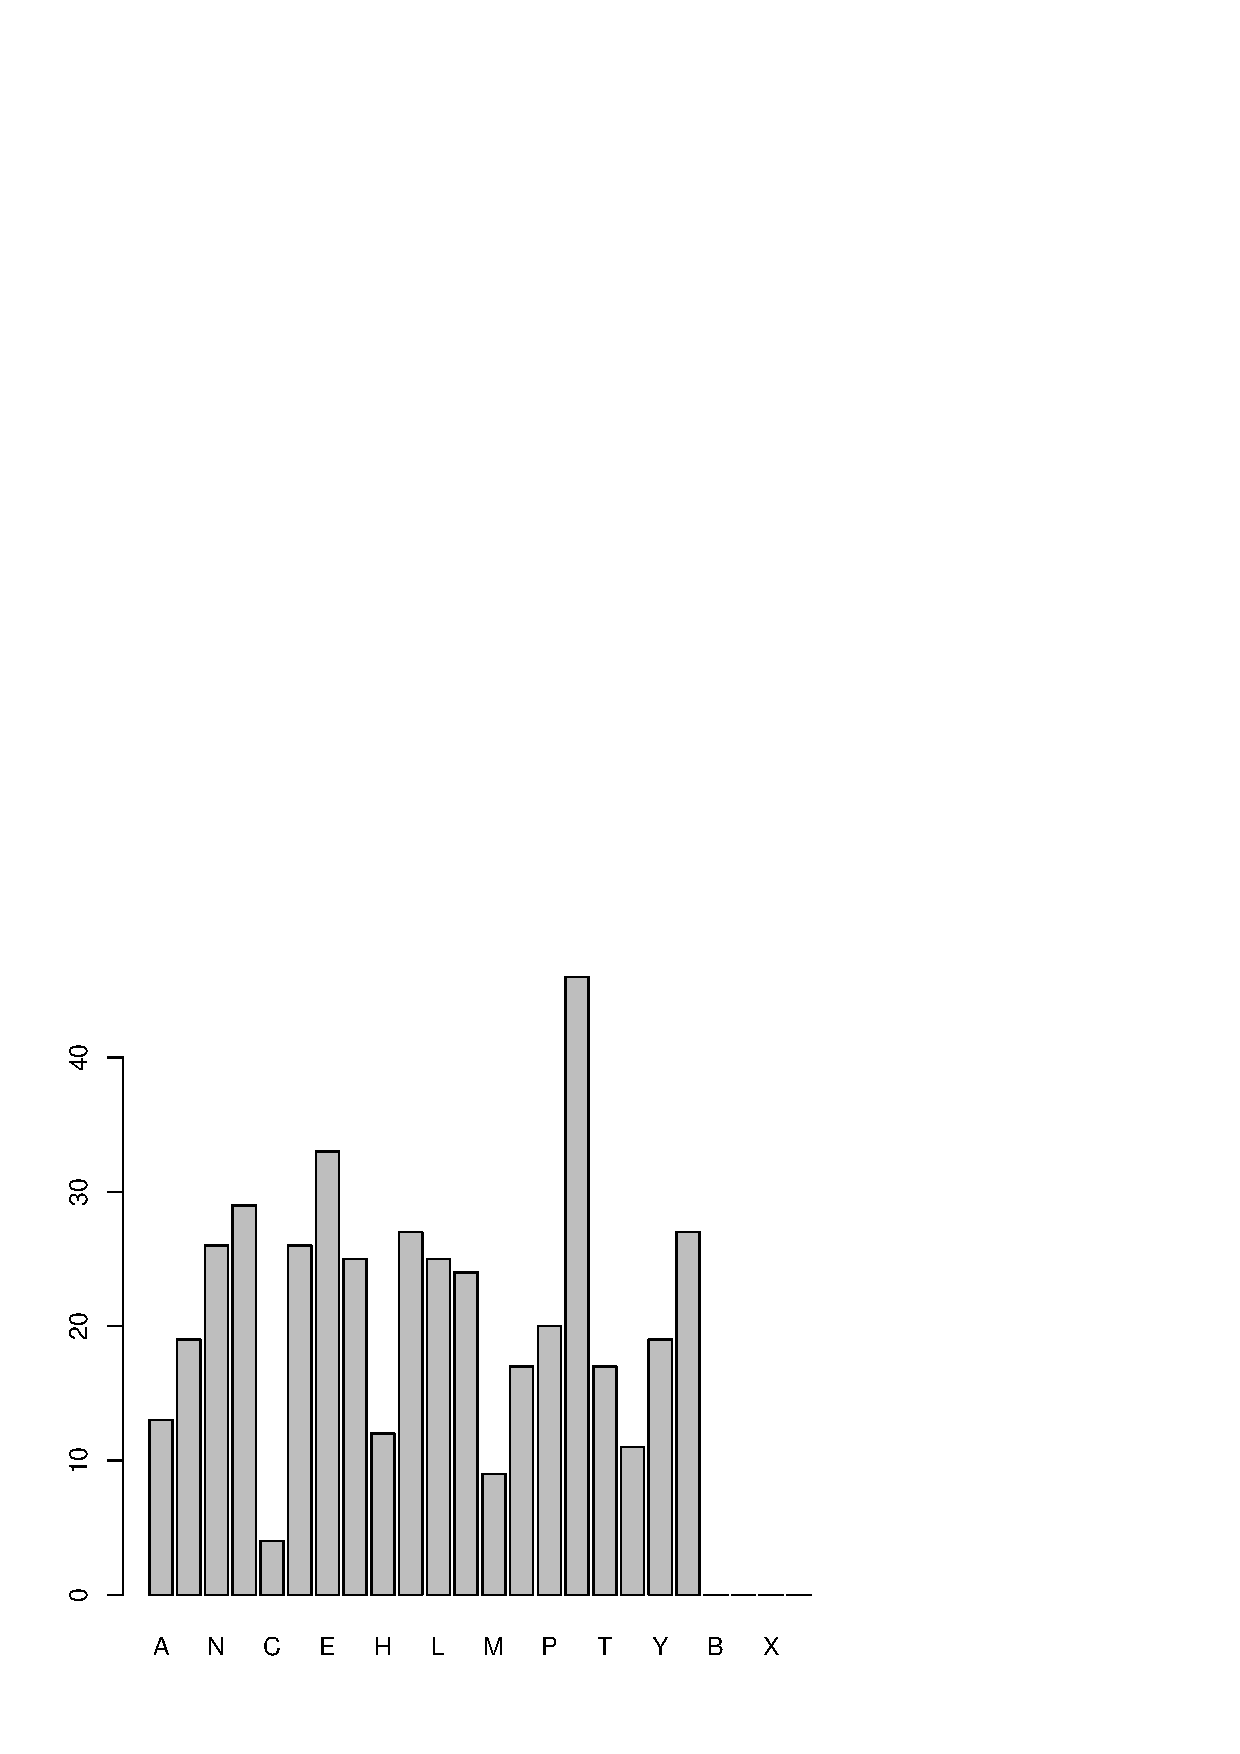
\includegraphics{SamplesSession-PlotAAFreq}

We also can compute a score if the sequence are aligned with itself.
To compute the alignment we also need a similarity matrix to judge the similarity between two amino acid residues and to compute an optimal alignment of the sequence. In the data directory you will find many different similarity matrices from the Emboss package.

\begin{Schunk}
\begin{Sinput}
> data(EPAM110)
> selfalign(mySequlist[[2]], EPAM110)
\end{Sinput}
\begin{Soutput}
  A 
738 
\end{Soutput}
\end{Schunk}

The class AASequence inherits from the R class character so you can use all the \texttt{R/base} functions defined for this class. E.g. to determine the length of the sequence we use the function \texttt{nchar}.

\begin{Schunk}
\begin{Sinput}
> nchar(mySequlist[[1]])
\end{Sinput}
\begin{Soutput}
[1] 429
\end{Soutput}
\end{Schunk}

For pairwise comparison of sequences we use the function \texttt{salign}. The parameters which control the behavior of the function are:
\begin{itemize}
\item \texttt{delta} = Gap opening penalty, (default = -4)
\item \texttt{gapext} = Gap extension penalty (default = delta)
\item \texttt{alignment} = Type of the alignment, either ``global'', ``local'', ``overlap'' alignment.
\item \texttt{scoring} = The return-type of the aligment. For two sequences it defaults to ``AAAlignment''.
\end{itemize}


The sequences in the sequence list can be accessed by their id. For two object of class \texttt{AASequence} the function \texttt{salign} returns by default an object of class ``AAAlignment''.
\begin{Schunk}
\begin{Sinput}
> str1 <- mySequlist[["At1g01580"]]
> str2 <- mySequlist[["At1g01590"]]
> as(str1, "character") <- substr(str1, 1, 90)
> as(str2, "character") <- substr(str2, 1, 140)
> res <- salign(str1, str2, EPAM110, delta = -4, gapext = -1, alignment = "global", 
+     scoring = "AAAlignment")
> res
\end{Sinput}
\begin{Soutput}
selfscore 1:  542 ; seq length 1 : 90 
selfscore 2:  821 ; seq length 2 : 140 
alig lenght:  153 
score      :  188 
FM         :  0.2818296 
identity   :  45 / 90 
similarity :  57 / 90 
\end{Soutput}
\end{Schunk}

To see how the sequences where aligned use the function \texttt{summary}. The ``|'' denotes a identity of amino acid residues, the ``:'' denotes a similarity.
\begin{Schunk}
\begin{Sinput}
> summary(res)
\end{Sinput}
\begin{Soutput}
selfscore 1:  542 
selfscore 2:  821 
alig lenght:  153 
score      :  188 
FM(score)  :  0.2818296 
identity   :  45 / 90 
similarity :  57 / 90 
At1g01580 MEIEKSNNGGSNPSAGEEFKDMI-KGVTKFLMMVIFLGTIMLWIMMPTLTYRTKWLPHLRI 
          |        |     ||  |::| | | ||||||| :|||::|||||| ||:  ||  :|  
At1g01590 M--------G----VGEMNKEVIDK-VIKFLMMVILMGTIVIWIMMPTSTYKEIWLTSMRA 

At1g01580 IKFGTSTYFGATGTTLFMYMFPMMVVA---C------------------------------ 
           | | | |:|  |  | :|||||:::|   |                               
At1g01590 AKLGKSIYYGRPGVNLLVYMFPMILLAFLGCIYLHLKKSTTVNQFNSGVEKKRAKFGALRR 

At1g01580 --------LGC---------------------- 
                  ||                        
At1g01590 RPMLVNGPLGIVTVTEVMFLTMFMALLLWSLAN 
\end{Soutput}
\end{Schunk}

\subsection{Scoring sequences}

We use the function align to score a sequence against a list of sequences for example to find the most similar sequence.
To rank the similarity of sequences we can use several scores.

\begin{itemize}
\item
Based on the number of identities (matches of identical amino acid residues) in the optimal alignment we define the \texttt{identity} as:
\begin{equation}
\frac{\textrm{\#identity}}{\textrm{length of shorter sequence}}
\end{equation}
\item 
Based on the number of similarities (similar amino acid residues at the same position in the alignment) we define the \texttt{similarity} as:
\begin{equation}
\frac{\textrm{\#similarity}}{\textrm{length of shorter sequence}}
\end{equation}

\item
The Smith Waterman, alignment \texttt{score} defined as:
\begin{equation}
S(A,B) = \sum^{N}_{k=1}{m_{{i_k}{j_k}}} - \textrm{gap penalties}
\end{equation}
\item
The normalized Smith Waterman alignment score (\texttt{scoreN}) we define as the score of the alignment (if it is larger 0) divided by the smaller score of the alignment of the sequences with itself, zero otherwise. 
\begin{eqnarray}
\frac{\textrm{score}}{\min(\textrm{selfscore 1},\textrm{selfscore 2})} \qquad \textrm{or 0 if score<0}
\end{eqnarray}

\item the \texttt{pozitive} score \cite{Booth}.
\begin{equation}
  POZ(A,B)=\frac{S(A,B)-\mu_{perm}}{\sigma_{perm}}
\end{equation}
\end{itemize}

To find a sequence in a list of sequences with the highest score to the bait sequence we use the function \texttt{salign} and \texttt{R/base} functions.

\begin{Schunk}
\begin{Sinput}
> sim1 <- salign(mySequlist, mySequlist[[1]], EPAM110, alignment = "global", 
+     scoring = "similarity")
> which(sim1 == max(sim1))
\end{Sinput}
\begin{Soutput}
At1g01010 
        1 
\end{Soutput}
\begin{Sinput}
> hist(sim1, breaks = 100)
\end{Sinput}
\end{Schunk}

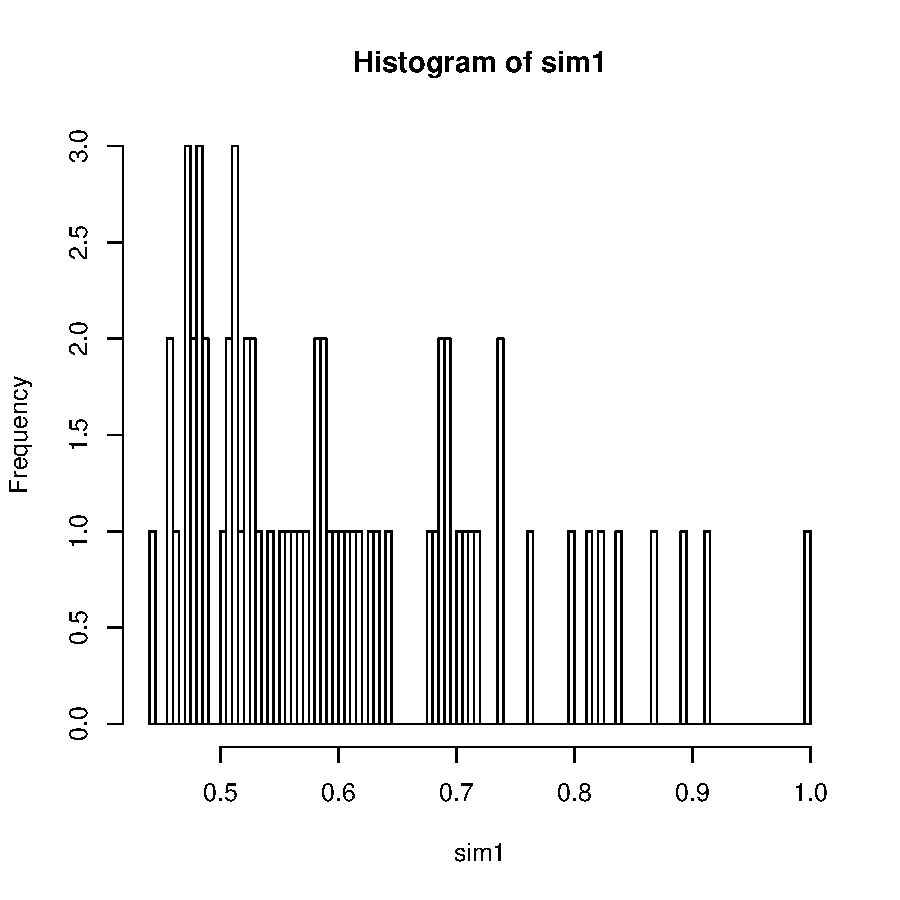
\includegraphics{SamplesSession-014}

We also use the function \texttt{salign} to compute a distance matrix for all sequences in the list. The distance matrix can be used for example for clustering. To obtain the distance matrix we supply a \texttt{AASequenceList} as first parameter and \texttt{NULL} as second parameter to the function \texttt{saling}. In this case the scores defined above are converted in distances:

\begin{itemize}
\item 1-\texttt{similarity}, 1-\texttt{identity}, 1-\texttt{scoreN}
\item Smith Waterman \texttt{score} first are converted into the Z score
\begin{equation}
  Z(A,B)=\frac{S(A,B)-\textrm{mean}}{\textrm{standard deviation}}
\end{equation}
Under the assumption that the Z scores for the sample set are normally distributed with {\em N(0,1)} \footnote{Its not\cite{Ving}! We do it, not to derive a significance of the alignment, but to transform the SW-score (or the pozitive score) into a distance measure and to cluster the dataset.} we compute the probability $P(X>= Z(A,B))$ that such or a higher score occur.
\item The POZITIVE score is as well transformed in a p-value $P(X >= Z_{pozitive})$ with the assumption that $X$ is normal distributed. 
\end{itemize}

\begin{Schunk}
\begin{Sinput}
> globaldist <- salign(mySequlist[1:10], NULL, EPAM110, alignment = "global", 
+     scoring = "score")
> localdist <- salign(mySequlist[1:10], NULL, EPAM110, alignment = "local", 
+     scoring = "score")
\end{Sinput}
\end{Schunk}

The distance matrix returned by the function \texttt{salign} can be supplied to many clustering algorithms provided by \texttt{R} e.g. to the hierarchical clustering function \texttt{hclust} in the package \texttt{R/mva}.

\begin{Schunk}
\begin{Sinput}
> plot(hclust(localdist))
\end{Sinput}
\end{Schunk}
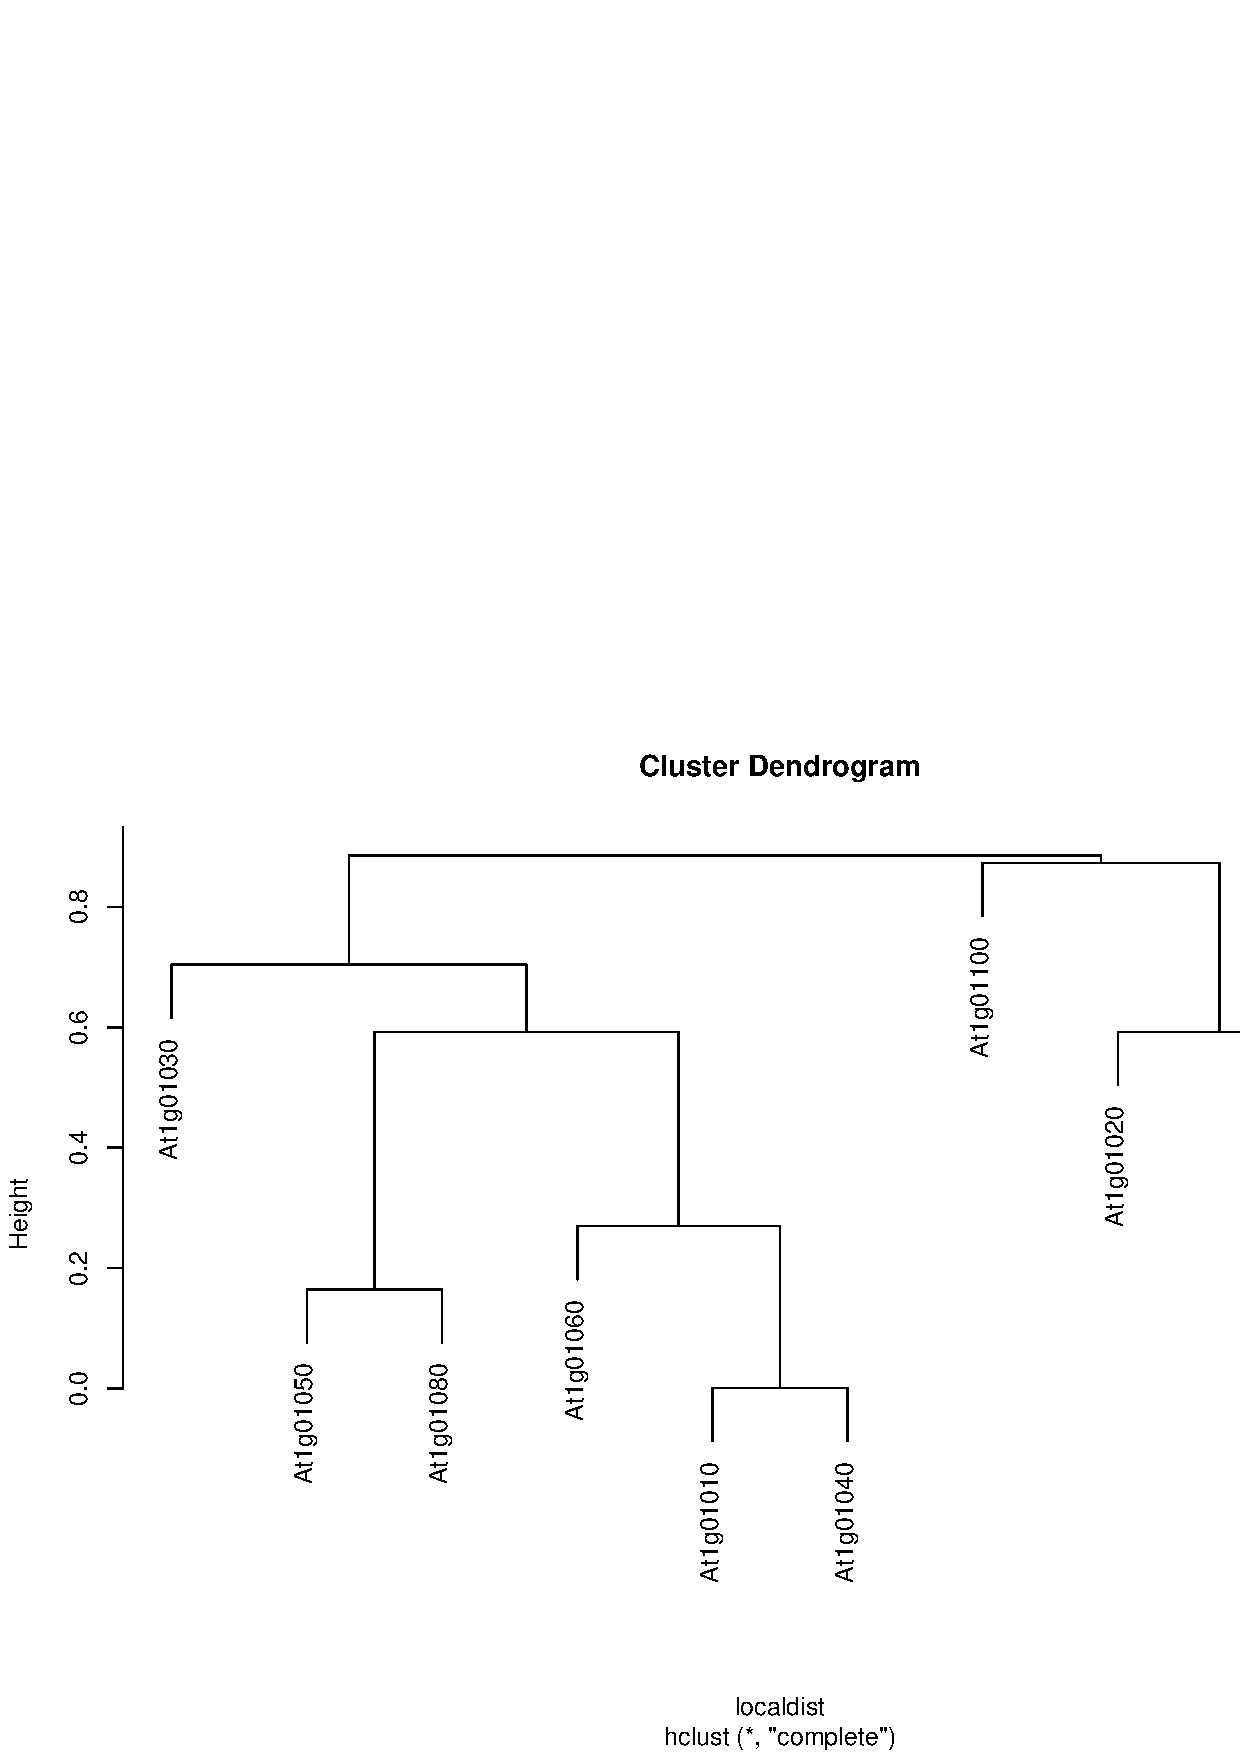
\includegraphics{SamplesSession-PlostClust}

It is also interesting to look at examples where the scores for different types of alignment highly differ. To do this the residues between the distance matrices can be computed and plotted
\begin{Schunk}
\begin{Sinput}
> plot(sort(as.numeric(localdist) - as.numeric(globaldist)), main = expression("Differences of the $P(Z_score)$ distance of local and overlap alignment"), 
+     xlab = "Sequence Pair", ylab = expression("Difference $P(Z_score)$"))
\end{Sinput}
\end{Schunk}
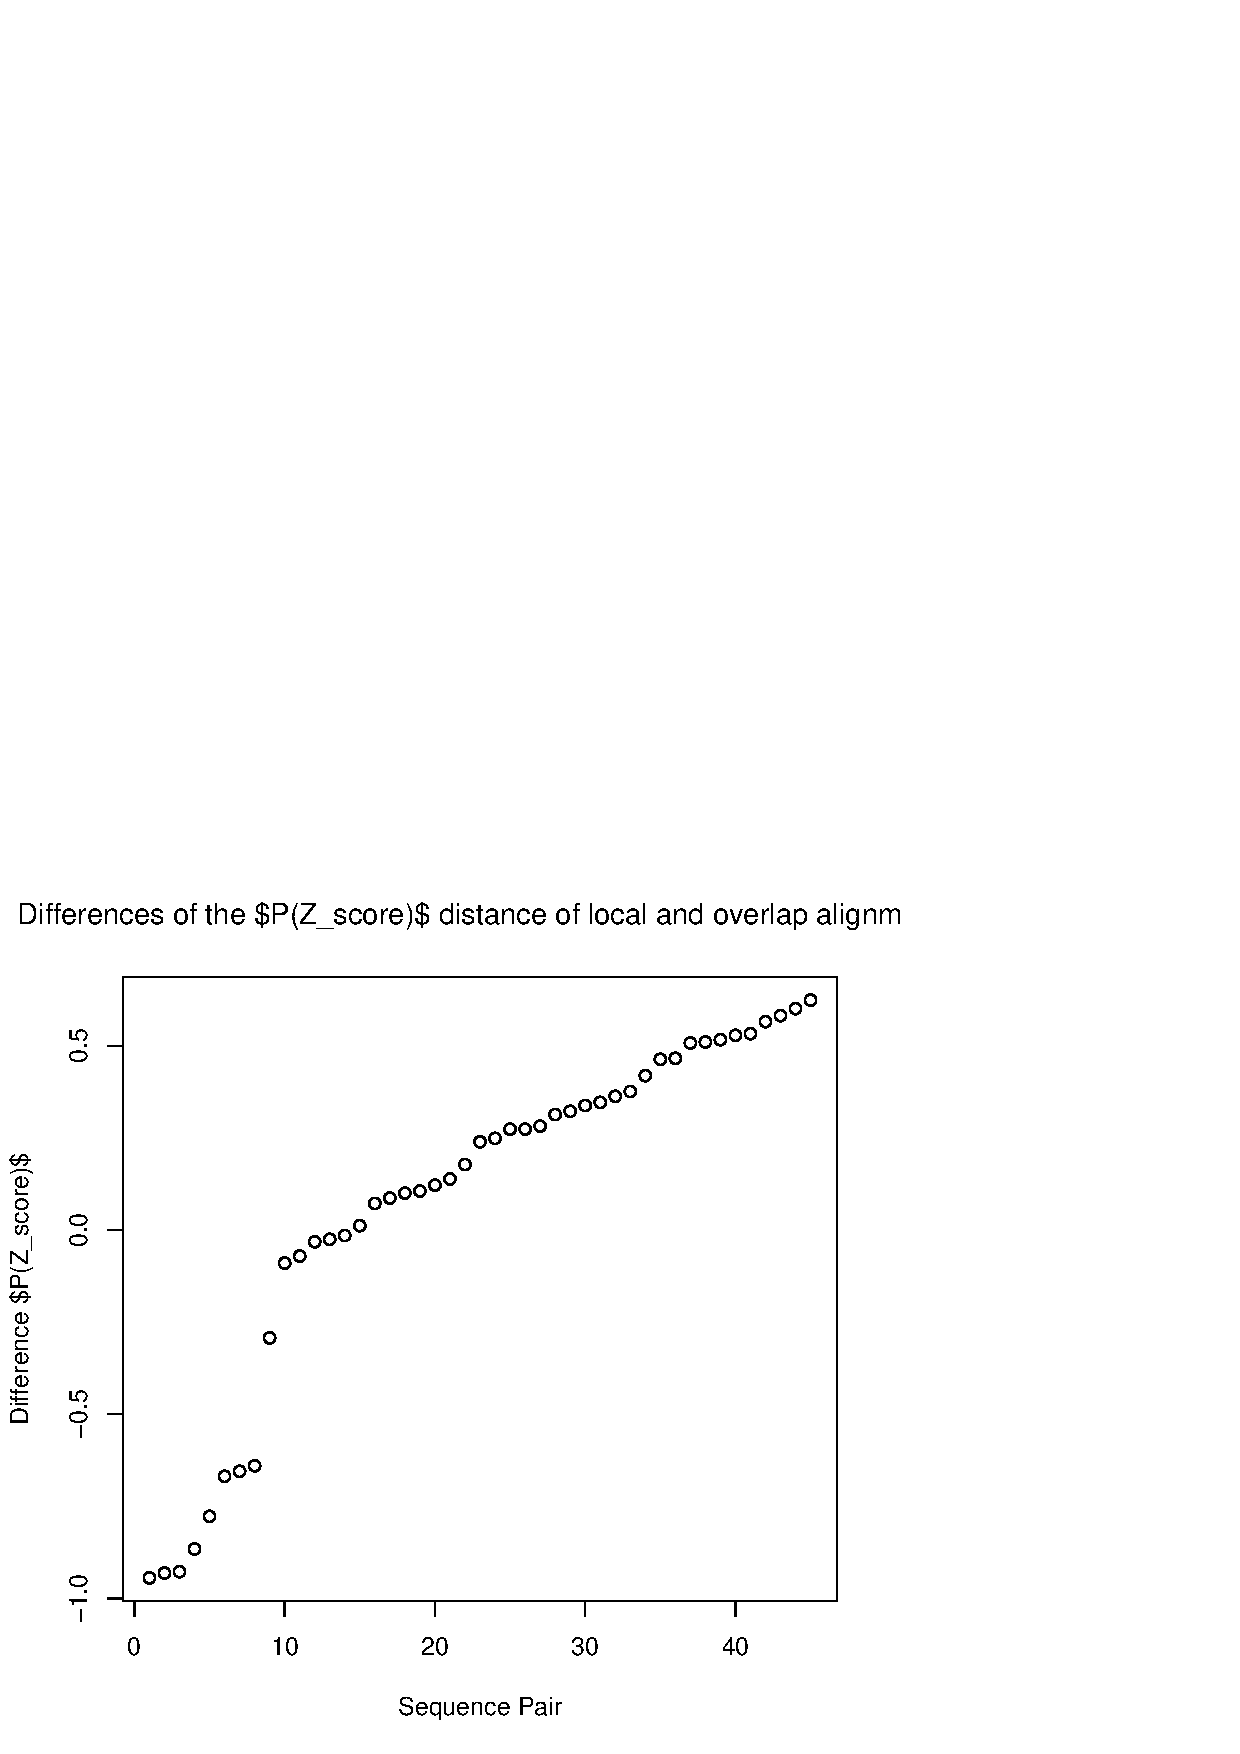
\includegraphics{SamplesSession-PlotResid}

We see that there are some sequence pairs which have different scores in the overlap and in the local alignment.

\section{Summary}

We are using the package \texttt{pairseqsim} to analyses results of Peptide Mass Fingerprint (PMF) identification experiments. By comparing the sequences of the highest scoring hits, we can draw conclusions about the significance of the identification result.
Have fun and let me know if you find errors(!), have suggestions, your impressions, or for what you found useful this tool.


\footnotesize
\begin{thebibliography}{99}
\bibitem{Booth}
Booth, H and Maindonald, J and  Nielsen, O and Wilson, S
Normalizing sequence alignment scores for composition bias
{\em Recomb 2003 - Berlin}
\bibitem{Ving}
Waterman, M. S. and Vingron, M. 1994. 
Sequence comparison significance and Poisson approximation. 
{\em Statistical Science}\texttt{9:367-381.}
\end{thebibliography}
\end{document}

